    \hypertarget{huxe9ritage-multiple}{%
\section{Héritage multiple}\label{huxe9ritage-multiple}}

    \hypertarget{compluxe9ment---niveau-intermuxe9diaire}{%
\subsection{Complément - niveau
intermédiaire}\label{compluxe9ment---niveau-intermuxe9diaire}}

    \hypertarget{la-classe-object}{%
\subsubsection{\texorpdfstring{La classe
\texttt{object}}{La classe object}}\label{la-classe-object}}

    Le symbole \texttt{object} est une variable prédéfinie (qui donc fait
partie du module \texttt{builtins})~:

    \begin{Verbatim}[commandchars=\\\{\}]
{\color{incolor}In [{\color{incolor}1}]:} \PY{n+nb}{object}
\end{Verbatim}


\begin{Verbatim}[commandchars=\\\{\}]
{\color{outcolor}Out[{\color{outcolor}1}]:} object
\end{Verbatim}
            
    \begin{Verbatim}[commandchars=\\\{\}]
{\color{incolor}In [{\color{incolor}2}]:} \PY{k+kn}{import} \PY{n+nn}{builtins}
        
        \PY{n}{builtins}\PY{o}{.}\PY{n}{object} \PY{o+ow}{is} \PY{n+nb}{object}
\end{Verbatim}


\begin{Verbatim}[commandchars=\\\{\}]
{\color{outcolor}Out[{\color{outcolor}2}]:} True
\end{Verbatim}
            
    La classe \texttt{object} est une classe spéciale~; toutes les classes
en Python héritent de la classe \texttt{object}, même lorsqu'aucun
héritage n'est spécifié~:

    \begin{Verbatim}[commandchars=\\\{\}]
{\color{incolor}In [{\color{incolor}3}]:} \PY{k}{class} \PY{n+nc}{Foo}\PY{p}{:}
            \PY{k}{pass}
        
        \PY{n}{Foo}\PY{o}{.}\PY{n+nv+vm}{\PYZus{}\PYZus{}bases\PYZus{}\PYZus{}}
\end{Verbatim}


\begin{Verbatim}[commandchars=\\\{\}]
{\color{outcolor}Out[{\color{outcolor}3}]:} (object,)
\end{Verbatim}
            
    L'attribut spécial \texttt{\_\_bases\_\_}, comme on le devine, nous
permet d'accéder aux superclasses directes, ici de la classe
\texttt{Foo}.\\

    En Python moderne, on n'a \textbf{jamais besoin de mentionner}
\texttt{object} dans le code. La raison de sa présence dans les symboles
prédéfinis est liée à l'histoire de Python, et à la distinction que
faisait Python 2 entre classes \emph{old-style} et classes
\emph{new-style}. Nous le mentionnons seulement car on rencontre encore
parfois du code qui fait quelque chose comme~:

    \begin{Verbatim}[commandchars=\\\{\}]
{\color{incolor}In [{\color{incolor}4}]:} \PY{k}{class} \PY{n+nc}{Bar}\PY{p}{(}\PY{n+nb}{object}\PY{p}{)}\PY{p}{:}
            \PY{k}{pass}
\end{Verbatim}


    qui est un reste de Python 2, et que Python 3 accepte uniquement au
titre de la compatibilité.

    \hypertarget{compluxe9ment---niveau-avancuxe9}{%
\subsection{Complément - niveau
avancé}\label{compluxe9ment---niveau-avancuxe9}}

    \hypertarget{rappels}{%
\subsubsection{Rappels}\label{rappels}}

    L'héritage en Python consiste principalement en l'algorithme de
recherche d'un attribut d'une instance~; celui-ci regarde~:

\begin{enumerate}
\def\labelenumi{\arabic{enumi}.}
\tightlist
\item
  d'abord dans l'instance~;
\item
  ensuite dans la classe~;
\item
  ensuite dans les super-classes.
\end{enumerate}

    \hypertarget{ordre-sur-les-super-classes}{%
\subsubsection{Ordre sur les
super-classes}\label{ordre-sur-les-super-classes}}

    Le problème revient donc, pour le dernier point, à définir un
\textbf{ordre} sur l'ensemble des \textbf{super-classes}. On parle bien,
naturellement, de \textbf{toutes} les super-classes, pas seulement
celles dont on hérite directement - en termes savants on dirait qu'on
s'intéresse à la fermeture transitive de la relation d'héritage.\\

L'algorithme utilisé pour cela depuis la version 2.3 est connu sous le
nom de \textbf{linéarisation C3}. Cet algorithme n'est pas propre à
python, comme vous pourrez le lire dans les références citées dans la
dernière section.\\

Nous ne décrirons pas ici l'algorithme lui-même dans le détail~; par
contre nous allons~:

\begin{itemize}
\tightlist
\item
  dans un premier temps résumer \textbf{les raisons} qui ont guidé ce
  choix, en décrivant les bonnes propriétés que l'on attend, ainsi que
  les \textbf{limitations} qui en découlent~;
\item
  puis voir l'ordre obtenu sur quelques \textbf{exemples} concrets de
  hiérarchies de classes.
\end{itemize}

Vous trouverez dans les références (voir ci-dessous la dernière section,
``Pour en savoir plus'') des liens vers des documents plus techniques si
vous souhaitez creuser le sujet.

    \hypertarget{les-bonnes-propriuxe9tuxe9s-attendues}{%
\subsubsection{Les bonnes propriétés
attendues}\label{les-bonnes-propriuxe9tuxe9s-attendues}}

    Il y a un certain nombre de bonnes propriétés que l'on attend de cet
algorithme.

    \hypertarget{priorituxe9-au-spuxe9cifique}{%
\subparagraph{Priorité au
spécifique\\\\}\label{priorituxe9-au-spuxe9cifique}}

    Lorsqu'une classe A hérite d'une classe B, on s'attend à ce que les
méthodes définies sur A, qui sont en principe plus spécifiques, soient
utilisées de préférence à celles définies sur B.

    \hypertarget{priorituxe9-uxe0-gauche}{%
\subparagraph{Priorité à gauche\\\\}\label{priorituxe9-uxe0-gauche}}

    Lorsqu'on utilise l'héritage multiple, on mentionne les classes mères
dans un certain ordre, qui n'est pas anodin. Les classes mentionnées en
premier sont bien entendu celles desquelles on veut hériter en priorité.

    \hypertarget{la-method-resolution-order-mro}{%
\section{La Method Resolution Order
(MRO)}\label{la-method-resolution-order-mro}}

    \hypertarget{de-maniuxe8re-un-peu-plus-formelle}{%
\subparagraph{De manière un peu plus
formelle\\\\}\label{de-maniuxe8re-un-peu-plus-formelle}}

    Pour reformuler les deux points ci-dessus, on s'intéresse à la
\texttt{mro} d'une classe O, et on veut avoir les deux bonnes propriétés
suivantes~:

\begin{itemize}
\tightlist
\item
  si O hérite (pas forcément directement) de A qui elle même hérite de
  B, alors A est avant B dans la \texttt{mro} de O~;
\item
  si O hérite (pas forcément directement) de A, qui elle hérite de B,
  puis (pas forcément immédiatement) de C, alors dans la \texttt{mro} A
  est avant B qui est avant C.
\end{itemize}

    \hypertarget{limitations-toutes-les-hiuxe9rarchies-ne-peuvent-pas-uxeatre-traituxe9es}{%
\subparagraph{Limitations~: toutes les hiérarchies ne peuvent pas être
traitées\\\\}\label{limitations-toutes-les-hiuxe9rarchies-ne-peuvent-pas-uxeatre-traituxe9es}}

    L'algorithme C3 permet de calculer un ordre sur \(\cal{S}\) qui respecte
toutes ces contraintes, lorsqu'il en existe un.\\

En effet, dans certains cas on ne peut pas trouver un tel ordre, on le
verra plus bas, mais dans la pratique, il est assez rare de tomber sur
de tels cas pathologiques~; et lorsque cela se produit c'est en général
le signe d'erreurs de conception plus profondes.

    \hypertarget{un-exemple-truxe8s-simple}{%
\subsubsection{Un exemple très simple}\label{un-exemple-truxe8s-simple}}

    On se donne la hiérarchie suivante~:

    \begin{Verbatim}[commandchars=\\\{\}]
{\color{incolor}In [{\color{incolor}5}]:} \PY{k}{class} \PY{n+nc}{LeftTop}\PY{p}{(}\PY{n+nb}{object}\PY{p}{)}\PY{p}{:}
            \PY{k}{def} \PY{n+nf}{attribut}\PY{p}{(}\PY{n+nb+bp}{self}\PY{p}{)}\PY{p}{:} 
                \PY{k}{return} \PY{l+s+s2}{\PYZdq{}}\PY{l+s+s2}{attribut(LeftTop)}\PY{l+s+s2}{\PYZdq{}}
            
        \PY{k}{class} \PY{n+nc}{LeftMiddle}\PY{p}{(}\PY{n}{LeftTop}\PY{p}{)}\PY{p}{:} 
            \PY{k}{pass}
        
        \PY{k}{class} \PY{n+nc}{Left}\PY{p}{(}\PY{n}{LeftMiddle}\PY{p}{)}\PY{p}{:} 
            \PY{k}{pass}
        
        \PY{k}{class} \PY{n+nc}{Middle}\PY{p}{(}\PY{n+nb}{object}\PY{p}{)}\PY{p}{:} 
            \PY{k}{pass}
        
        \PY{k}{class} \PY{n+nc}{Right}\PY{p}{(}\PY{n+nb}{object}\PY{p}{)}\PY{p}{:}
            \PY{k}{def} \PY{n+nf}{attribut}\PY{p}{(}\PY{n+nb+bp}{self}\PY{p}{)}\PY{p}{:} 
                \PY{k}{return} \PY{l+s+s2}{\PYZdq{}}\PY{l+s+s2}{attribut(Right)}\PY{l+s+s2}{\PYZdq{}}
        
        \PY{k}{class} \PY{n+nc}{Class}\PY{p}{(}\PY{n}{Left}\PY{p}{,} \PY{n}{Middle}\PY{p}{,} \PY{n}{Right}\PY{p}{)}\PY{p}{:} 
            \PY{k}{pass}
        
        \PY{n}{instance} \PY{o}{=} \PY{n}{Class}\PY{p}{(}\PY{p}{)}
\end{Verbatim}


    qui donne en version dessinée, avec deux points rouges pour représenter
les deux définitions de la méthode \texttt{attribut}~:

    Les deux règles, telles que nous les avons énoncées en premier lieu
(priorité à gauche, priorité au spécifique) sont un peu contradictoires
ici. En fait, c'est la méthode de \texttt{LeftTop} qui est héritée dans
\texttt{Class}, comme on le voit ici~:\\

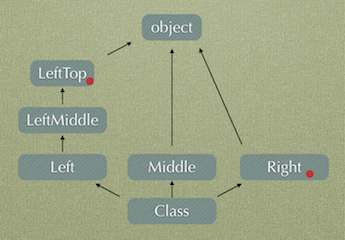
\includegraphics{medias/heritage-multiple01.png}

    \begin{Verbatim}[commandchars=\\\{\}]
{\color{incolor}In [{\color{incolor}6}]:} \PY{n}{instance}\PY{o}{.}\PY{n}{attribut}\PY{p}{(}\PY{p}{)} \PY{o}{==} \PY{l+s+s1}{\PYZsq{}}\PY{l+s+s1}{attribut(LeftTop)}\PY{l+s+s1}{\PYZsq{}}
\end{Verbatim}


\begin{Verbatim}[commandchars=\\\{\}]
{\color{outcolor}Out[{\color{outcolor}6}]:} True
\end{Verbatim}
            
    \textbf{Exercice}~: Remarquez qu'ici \texttt{Right} a elle-même un
héritage très simple. À titre d'exercice, modifiez le code ci-dessus
pour faire que \texttt{Right} hérite de la classe \texttt{LeftMiddle}~;
de quelle classe d'après vous est-ce que \texttt{Class} hérite
\texttt{attribut} dans cette configuration~?

    \hypertarget{si-cela-ne-vous-convient-pas}{%
\subparagraph{Si cela ne vous convient
pas\\\\}\label{si-cela-ne-vous-convient-pas}}

    C'est une évidence, mais cela va peut-être mieux en le rappelant~: si la
méthode que vous obtenez ``gratuitement'' avec l'héritage n'est pas
celle qui vous convient, vous avez naturellement toujours la possibilité
de la redéfinir, et ainsi d'en \textbf{choisir} une autre. Dans notre
exemple si on préfère la méthode implémentée dans \texttt{Right}, on
définira plutôt la classe \texttt{Class} comme ceci~:

    \begin{Verbatim}[commandchars=\\\{\}]
{\color{incolor}In [{\color{incolor}7}]:} \PY{k}{class} \PY{n+nc}{Class}\PY{p}{(}\PY{n}{Left}\PY{p}{,} \PY{n}{Middle}\PY{p}{,} \PY{n}{Right}\PY{p}{)}\PY{p}{:}
            \PY{c+c1}{\PYZsh{} en redéfinissant explicitement la méthode}
            \PY{c+c1}{\PYZsh{} attribut ici on court\PYZhy{}circuite la mro}
            \PY{c+c1}{\PYZsh{} et on peut appeler explicitement une autre}
            \PY{c+c1}{\PYZsh{} version de attribut()}
            \PY{k}{def} \PY{n+nf}{attribut}\PY{p}{(}\PY{o}{*}\PY{n}{args}\PY{p}{,} \PY{o}{*}\PY{o}{*}\PY{n}{kwds}\PY{p}{)}\PY{p}{:}
                \PY{k}{return} \PY{n}{Right}\PY{o}{.}\PY{n}{attribut}\PY{p}{(}\PY{o}{*}\PY{n}{args}\PY{p}{,} \PY{o}{*}\PY{o}{*}\PY{n}{kwds}\PY{p}{)}
            
        \PY{n}{instance2} \PY{o}{=} \PY{n}{Class}\PY{p}{(}\PY{p}{)}
        \PY{n}{instance2}\PY{o}{.}\PY{n}{attribut}\PY{p}{(}\PY{p}{)}
\end{Verbatim}


\begin{Verbatim}[commandchars=\\\{\}]
{\color{outcolor}Out[{\color{outcolor}7}]:} 'attribut(Right)'
\end{Verbatim}
            
    Ou encore bien entendu, si dans votre contexte vous devez appelez
\textbf{les deux} méthodes dont vous pourriez hériter et les combiner,
vous pouvez le faire aussi, par exemple comme ceci~:

    \begin{Verbatim}[commandchars=\\\{\}]
{\color{incolor}In [{\color{incolor}8}]:} \PY{k}{class} \PY{n+nc}{Class}\PY{p}{(}\PY{n}{Left}\PY{p}{,} \PY{n}{Middle}\PY{p}{,} \PY{n}{Right}\PY{p}{)}\PY{p}{:}
            \PY{c+c1}{\PYZsh{} pour faire un composite des deux méthodes}
            \PY{c+c1}{\PYZsh{} trouvées dans les classes mères}
            \PY{k}{def} \PY{n+nf}{attribut}\PY{p}{(}\PY{o}{*}\PY{n}{args}\PY{p}{,} \PY{o}{*}\PY{o}{*}\PY{n}{kwds}\PY{p}{)}\PY{p}{:}
                \PY{k}{return} \PY{n}{LeftTop}\PY{o}{.}\PY{n}{attribut}\PY{p}{(}\PY{o}{*}\PY{n}{args}\PY{p}{,} \PY{o}{*}\PY{o}{*}\PY{n}{kwds}\PY{p}{)} \PY{o}{+}
                 \PY{l+s+s2}{\PYZdq{}}\PY{l+s+s2}{ ** }\PY{l+s+s2}{\PYZdq{}} \PY{o}{+} \PY{n}{Right}\PY{o}{.}\PY{n}{attribut}\PY{p}{(}\PY{o}{*}\PY{n}{args}\PY{p}{,} \PY{o}{*}\PY{o}{*}\PY{n}{kwds}\PY{p}{)} 
            
        \PY{n}{instance3} \PY{o}{=} \PY{n}{Class}\PY{p}{(}\PY{p}{)}
        \PY{n}{instance3}\PY{o}{.}\PY{n}{attribut}\PY{p}{(}\PY{p}{)}
\end{Verbatim}


\begin{Verbatim}[commandchars=\\\{\}]
{\color{outcolor}Out[{\color{outcolor}8}]:} 'attribut(LeftTop) ** attribut(Right)'
\end{Verbatim}
            
    \hypertarget{un-exemple-un-peu-plus-compliquuxe9}{%
\subsubsection{Un exemple un peu plus
compliqué}\label{un-exemple-un-peu-plus-compliquuxe9}}

    Voici un exemple, assez parlant, tiré de la deuxième référence (voir
ci-dessous la dernière section, ``Pour en savoir plus'').

    \begin{Verbatim}[commandchars=\\\{\}]
{\color{incolor}In [{\color{incolor}9}]:} \PY{n}{O} \PY{o}{=} \PY{n+nb}{object}
        \PY{k}{class} \PY{n+nc}{F}\PY{p}{(}\PY{n}{O}\PY{p}{)}\PY{p}{:} \PY{k}{pass}
        \PY{k}{class} \PY{n+nc}{E}\PY{p}{(}\PY{n}{O}\PY{p}{)}\PY{p}{:} \PY{k}{pass}
        \PY{k}{class} \PY{n+nc}{D}\PY{p}{(}\PY{n}{O}\PY{p}{)}\PY{p}{:} \PY{k}{pass}
        \PY{k}{class} \PY{n+nc}{C}\PY{p}{(}\PY{n}{D}\PY{p}{,} \PY{n}{F}\PY{p}{)}\PY{p}{:} \PY{k}{pass}
        \PY{k}{class} \PY{n+nc}{B}\PY{p}{(}\PY{n}{E}\PY{p}{,} \PY{n}{D}\PY{p}{)}\PY{p}{:} \PY{k}{pass}
        \PY{k}{class} \PY{n+nc}{A}\PY{p}{(}\PY{n}{B}\PY{p}{,} \PY{n}{C}\PY{p}{)}\PY{p}{:} \PY{k}{pass}
\end{Verbatim}


    Cette hiérarchie nous donne, en partant de A, l'ordre suivant~:

    \begin{verbatim}
                           6
                          ---
Level 3                  | O |
                       /  ---  \
                      /    |    \
                     /     |     \
                    /      |      \
                  ---     ---    ---
Level 2        2 | E | 4 | D |  | F | 5
                  ---     ---    ---
                   \      / \     /
                    \    /   \   /
                     \  /     \ /
                      ---     ---
Level 1            1 | B |   | C | 3
                      ---     ---
                       \       /
                        \     /
                          ---
Level 0                0 | A |
                          ---
\end{verbatim}

    Que l'on peut calculer, sous l'interpréteur python, avec la méthode
\texttt{mro} sur la classe de départ~:

    \begin{Verbatim}[commandchars=\\\{\}]
{\color{incolor}In [{\color{incolor}10}]:} \PY{n}{A}\PY{o}{.}\PY{n}{mro}\PY{p}{(}\PY{p}{)}
\end{Verbatim}


\begin{Verbatim}[commandchars=\\\{\}]
{\color{outcolor}Out[{\color{outcolor}10}]:} [\_\_main\_\_.A,
          \_\_main\_\_.B,
          \_\_main\_\_.E,
          \_\_main\_\_.C,
          \_\_main\_\_.D,
          \_\_main\_\_.F,
          object]
\end{Verbatim}
            
    \hypertarget{un-exemple-qui-ne-peut-pas-uxeatre-traituxe9}{%
\subsubsection{Un exemple qui ne peut pas être
traité}\label{un-exemple-qui-ne-peut-pas-uxeatre-traituxe9}}

    Voici enfin un exemple de hiérarchie pour laquelle on ne \textbf{peut
pas trouver d'ordre} qui respecte les bonnes propriétés que l'on a vues
tout à l'heure, et qui pour cette raison sera \textbf{rejetée par
l'interpréteur python}. D'abord en version dessinée~:\\

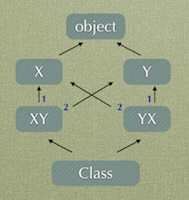
\includegraphics{medias/heritage-multiple02.png}

    \begin{Verbatim}[commandchars=\\\{\}]
{\color{incolor}In [{\color{incolor}11}]:} \PY{c+c1}{\PYZsh{} puis en version code}
         \PY{k}{class} \PY{n+nc}{X}\PY{p}{:} \PY{k}{pass}
         \PY{k}{class} \PY{n+nc}{Y}\PY{p}{:} \PY{k}{pass}
         \PY{k}{class} \PY{n+nc}{XY}\PY{p}{(}\PY{n}{X}\PY{p}{,} \PY{n}{Y}\PY{p}{)}\PY{p}{:} \PY{k}{pass}
         \PY{k}{class} \PY{n+nc}{YX}\PY{p}{(}\PY{n}{Y}\PY{p}{,} \PY{n}{X}\PY{p}{)}\PY{p}{:} \PY{k}{pass}
         
         \PY{c+c1}{\PYZsh{} on essaie de créer une sous\PYZhy{}classe de XY et YX}
         \PY{k}{try}\PY{p}{:}
             \PY{k}{class} \PY{n+nc}{Class}\PY{p}{(}\PY{n}{XY}\PY{p}{,} \PY{n}{YX}\PY{p}{)}\PY{p}{:} \PY{k}{pass} 
         \PY{c+c1}{\PYZsh{} mais ce n\PYZsq{}est pas possible}
         \PY{k}{except} \PY{n+ne}{Exception} \PY{k}{as} \PY{n}{e}\PY{p}{:}
             \PY{n+nb}{print}\PY{p}{(}\PY{n}{f}\PY{l+s+s2}{\PYZdq{}}\PY{l+s+s2}{OOPS, }\PY{l+s+s2}{\PYZob{}}\PY{l+s+s2}{type(e)\PYZcb{}, }\PY{l+s+si}{\PYZob{}e\PYZcb{}}\PY{l+s+s2}{\PYZdq{}}\PY{p}{)}
\end{Verbatim}


    \begin{Verbatim}[commandchars=\\\{\}]
OOPS, <class 'TypeError'>, Cannot create a consistent method resolution
order (MRO) for bases X, Y

    \end{Verbatim}

    \hypertarget{pour-en-savoir-plus}{%
\subsubsection{Pour en savoir plus}\label{pour-en-savoir-plus}}

    \begin{enumerate}
\def\labelenumi{\arabic{enumi}.}
\setcounter{enumi}{-1}
\tightlist
\item
  Un
  \href{http://python-history.blogspot.fr/2010/06/method-resolution-order.html}{blog
  de Guido Van Rossum} qui retrace l'historique des différents essais
  qui ont été faits avant de converger sur le modèle actuel.
\item
  Un \href{https://www.python.org/download/releases/2.3/mro/}{article
  technique} qui décrit le fonctionnement de l'algorithme de calcul de
  la MRO, et donne des exemples.
\item
  L'\href{http://en.wikipedia.org/wiki/C3_linearization}{article de
  Wikipedia} sur l'algorithme C3.
\end{enumerate}